\section{Обсуждение результатов}

Из численных результатов (рис.~\ref{img:res_comparison}) было получено, что верхняя граница применимости плазмонной линейки в случае резонанса первого порядка составляет $ \approx 170 \pm 10 $~нм, а в случае резонанса второго порядка она больше и составляет $ \approx 370 \pm 10 $~нм. Из экспериментальных данных мы видим, что для резонанса ЛПП второго порядка экспериментальная кривая положения резонанса ЛПП от расстояния между наностержнями согласуется с численными расчетами за исключением того, что в абсолютных значениях экспериментально полученные данные положения резонанса ЛПП сдвинуты в красную область на  $ \approx 25 $~нм в случае длины наностержней $ a = $ 400~нм и на $ \approx 50 $~нм в случае длины наностержней $ a = $ 500~нм. Это связано с тем, что численном расчете не учитывалась кварцевая подложка, которая влияет на положение резонанса ЛПП. В случае резонанса первого порядка ЛПП экспериментальные данные не согласуются с численными расчетами (рис.~\ref{img:1res}). Это связано с дифракцией излучения на периодически расположенных $ \pi $-димерах в исследуемых образцах. В случае же численного эксперимента при расчете зависимости положения резонанса ЛПП от расстояния между наностержнями использовались граничные условия PML, которые с физической точки зрения поглощают все падающее на них электромагнитное поле.
\begin{figure}
\center{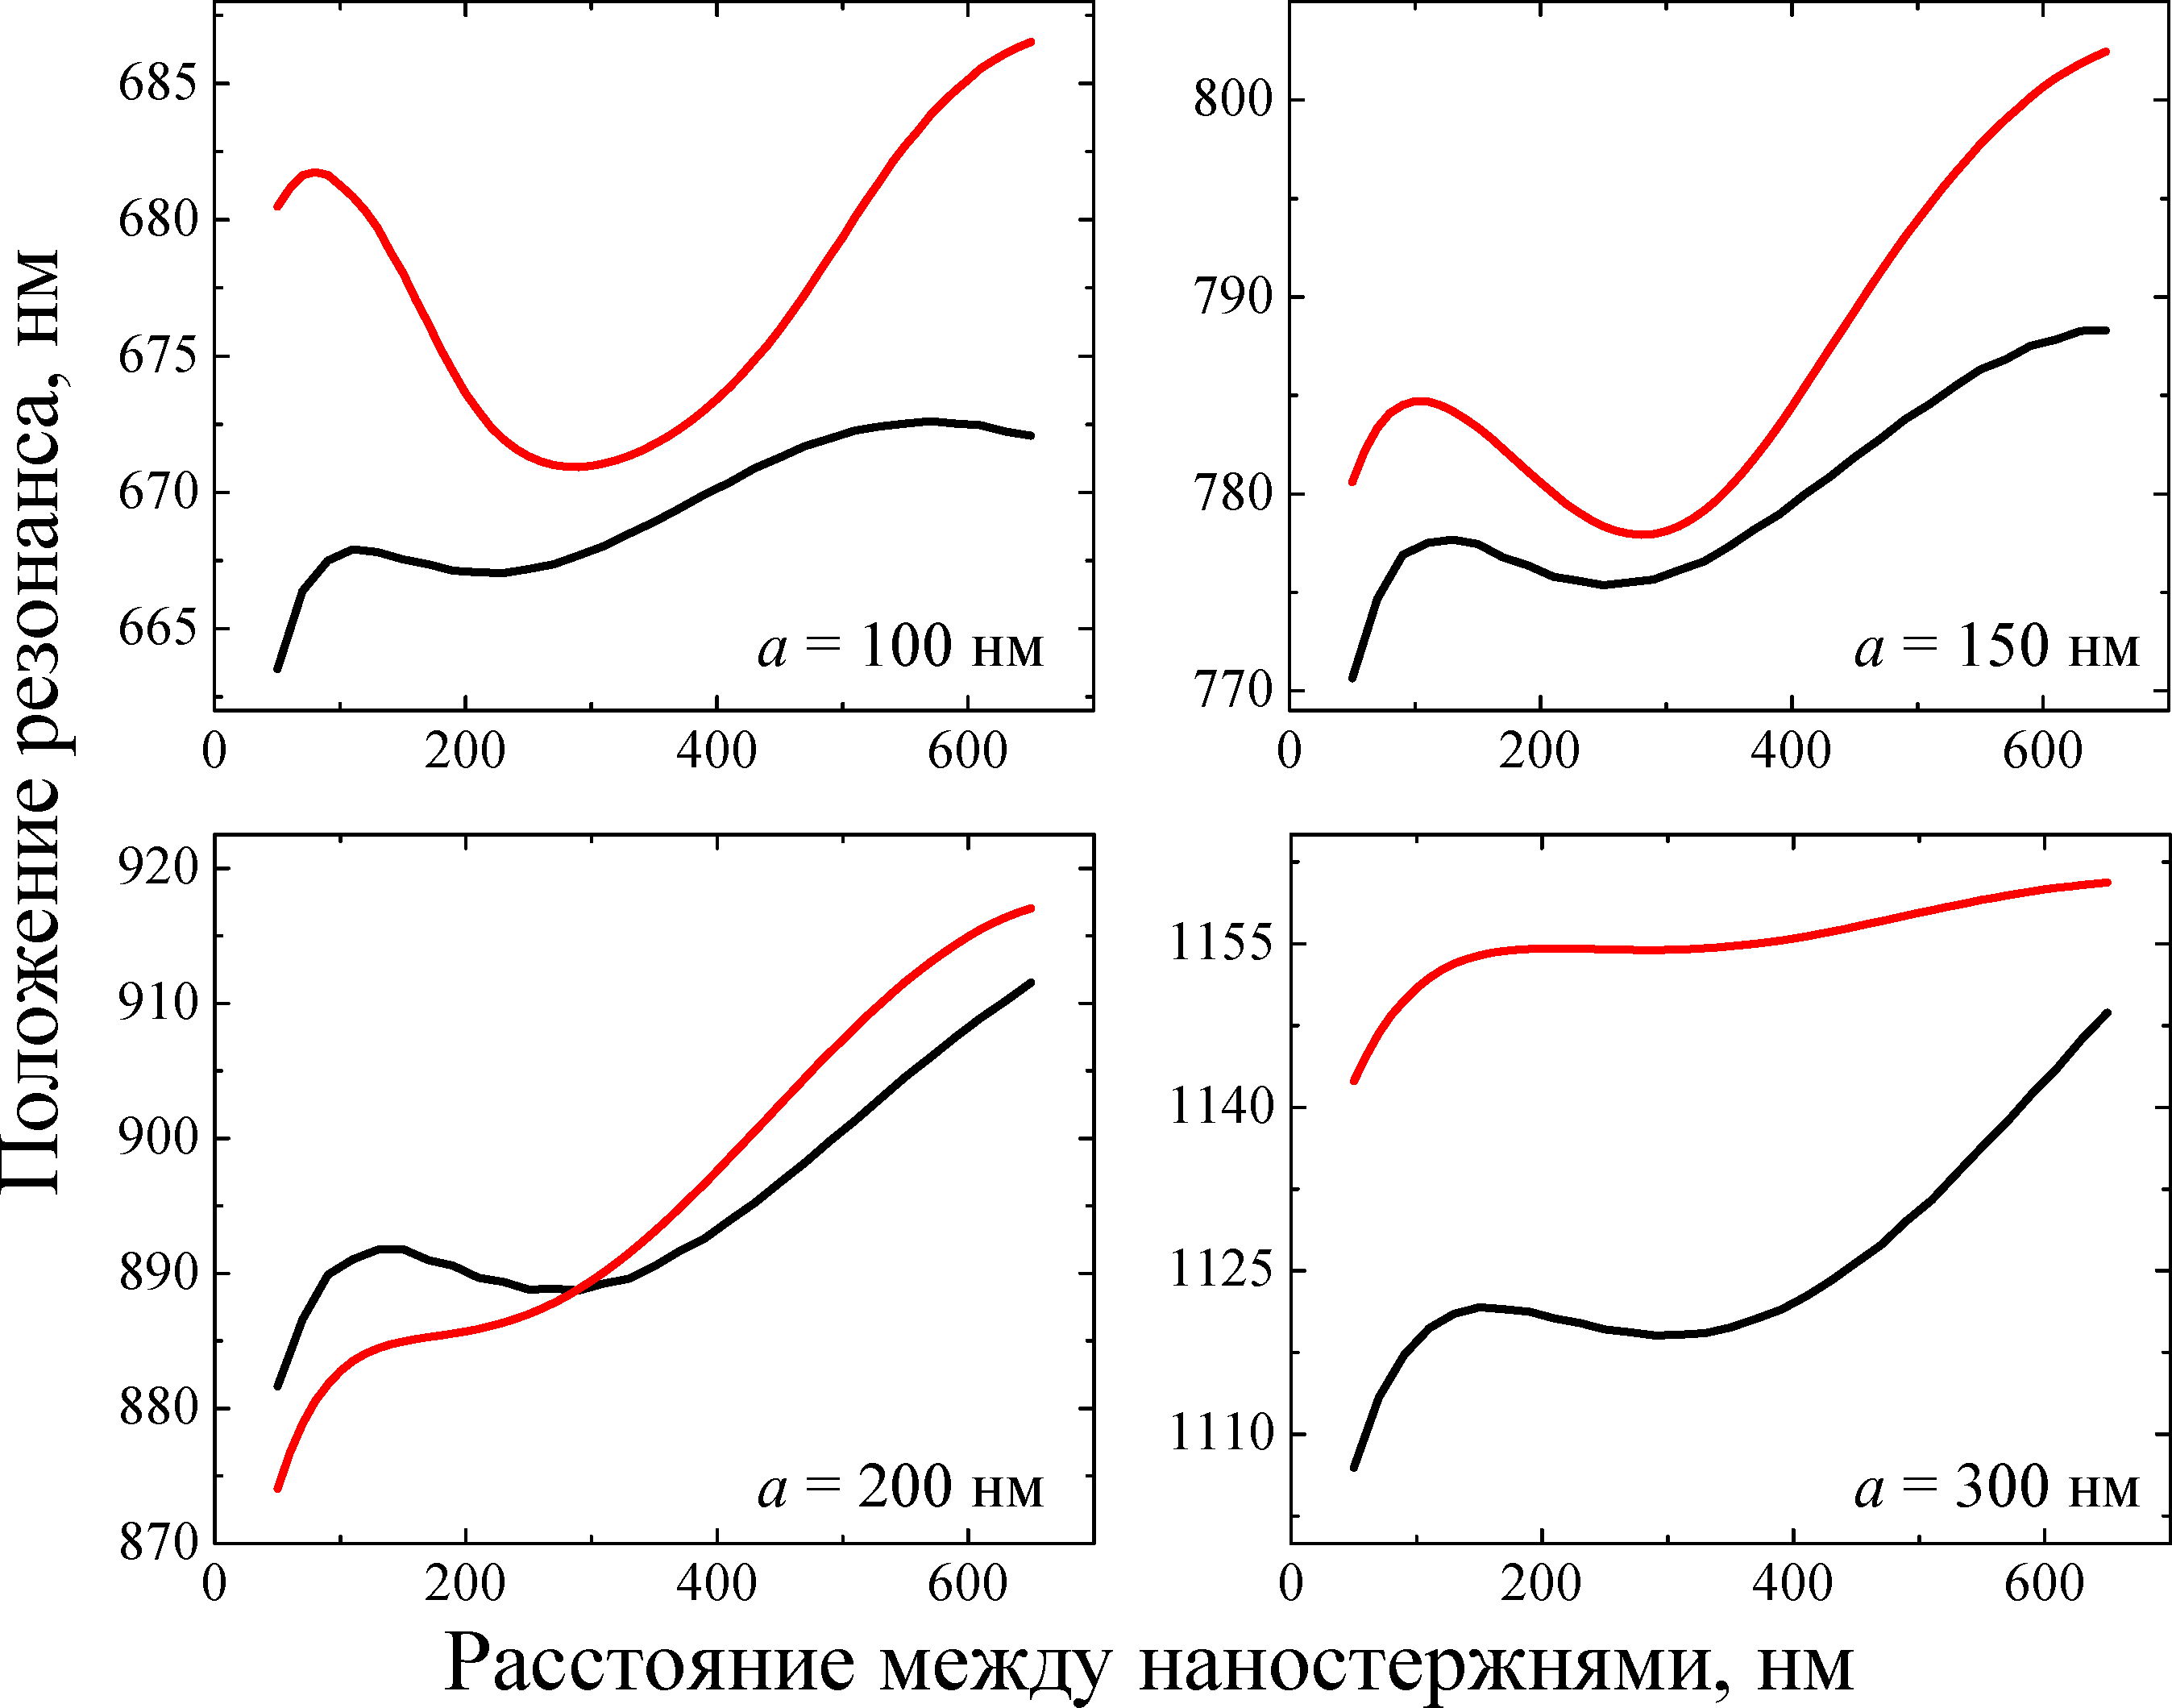
\includegraphics[width=0.7\linewidth]{img/analytics/res_PML_periodic.pdf}}
\caption{Численно рассчитанная зависимость положения резонанса ЛПП от расстояния между наностержнями в случае периодических граничных условий (красная кривая) и в случае условий PML (черная кривая) для $ \pi $-димеров с длиной наностержней $ a = $ 100, 150, 200 и 300~нм.}
\label{img:res_PML_periodic}
\end{figure}
Поэтому при расчете зависимости положения резонанса ЛПП от расстояния между наностержнями граничные условия PML были изменены на периодические граничные условия. На рис.~\ref{img:res_PML_periodic} показана рассчитанная численно зависимость положения резонанса ЛПП в случае периодических граничных условия (красная кривая) и условий PML (черная кривая). Видно, что дифракционное взаимодействие влияет и на период осцилляций положения резонанса, и на его модуляцию.
Для того, чтобы учесть периодичность структуры были проведены численные расчеты спектров коэффициента экстинкции для $ \pi $-димеров с фиксированной длиной наностержней $ a = $ 300~нм и расстоянием между наностержнями $ d = $ 300~нм от расстояния между $ \pi $-димерами (рис.~\ref{img:BCperiod}). Видно, что резонанс второго порядка менее чувствителен к периоду между $ \pi $-димерами, в то время как положение резонанса первого порядка начинает сильно изменяться из-за дифракционного взаимодействия между $ \pi $-димерами, а иногда происходит расщепление резонанса ЛПП первого порядка. Аналогичный эффект дифракционного взаимодействия наблюдался в случае периодически расположенных наноантенн в работе \cite{diffractionCoupling}. Наноантенны представляли собой нанокольца, и наблюдалось два резонанса: дипольный и квадрупольный. Квадрупольный резонанс оказался менее чувствителен к дифракционному взаимодействию наноантенн. В нашем случае было показано, что резонанс ЛПП первого порядка сильнее связан с плоскими волнами, как показано на спектре пропускания на рис.~\ref{img:spectraFDTDa500d100}, что говорит о его большей чувствительности к дальнепольному (в том числе дифракционному) взаимодействию.
Таким образом, дальнепольное взаимодействие между наностержнями в димере приводят к тому, что верхняя граница применимости $ \pi $-димера в качестве плазмонной линейки в случае резонанса первого порядка меньше, чем для резонанса второго порядка, а дифракционное взаимодействие делает невозможным использование резонанса ЛПП первого порядка в качестве плазмонной линейки.